
\chapter{Theory}
The purpose of this chapter is to explain the mathematical concepts behind the numerical models used and to provide useful insight into the working concepts of the algorithms developed. Initially, the constraints defining a techno-economic energy model is presented to provide a good understanding of the optimization problem. Next, the working principles of existing MGA algorithms are presented, as they serve as the foundation for the MGA method developed in this project. 

In this project, the following mathematical formulations will be used. Scalar values will be non-bold characters such as $d$. Vectors will be represented by bold characters $ \mathbf{x} $. Single values in a vector are indexed using a subscript $ \mathbf{x}_i $, as in this example where the $i$'th element of $\mathbf{x}$ is represented. Vectors of higher dimensions will be indexed with as many variables as dimensions. For example, a single value from a three-dimensional vector may be accessed as $\mathbf{g}_{n,s,t}$. A specific point given as a vector is indexed with superscript such that  $\mathbf{x}^1$, refers to a specific configuration of $\mathbf{x}$. Sets will be assigned non-bold capital letters such as $W$. 

\section{Techno-Economic model mathematical formulation}\label{sec:OptimizationProblem}

To fully understand the techno-economic model, the mathematical formulation of the model must first be understood. In this section, the objective function and the constraints defining the numeric techno-economic model will be presented and explained. 

The goal is to formulate the techno-economic model in the form of a classic optimization problem as explained in \cite{ConvexOpimization}, where an objective function is defined along with a set of constraints on the form presented in Equation \ref{eq:ConvexOptimization}. All constraints are collected in the vector functions  $\mathbf{f}_i$ and $\mathbf{h}_i$, and are rewritten to be either less than or equal to $0$. The vector $\mathbf{x} \subseteq \mathbb{R}^d$ contain the optimization variables to be optimized. 

\begin{equation}\label{eq:ConvexOptimization}
\begin{split}
\text{minimize} \;&\; \mathbf{f}_0(\mathbf{x})   \; \\
\text{subject to} \; &\; \mathbf{f}_i(\mathbf{x}) \leq 0 \; \; i=1..m\\
\;            &\;  \mathbf{h}_i(\mathbf{x}) = 0 \; \; i=1..p\\
\end{split}
\end{equation}

It is possible to formulate the techno-economic optimization problem in this form by studying the individual components of the model and defining their individual relations with constraints. But first of all the components in the techno-economic model must be identified. 

The techno-economic energy model is built as a network where each country is represented as a node connected to the surrounding countries through a link. Each country/node has three energy-producing technologies available, gas turbines (OCGT), wind turbines, solar PV and an energy load that must be satisfied. In the model a range of snapshots is defined, each representing an hour of the year. For each hour all energy demands must be satisfied and to do so the installed capacities of the available technologies can be increased if necessary, at the expense of added system cost. 

Following the naming convention from \cite{PyPSA_euro_30_model}, indexing the nodes in the network with the variable $n$, the power generating technologies by $s$, the hours in the year by $t$ and the possible connecting power lines by $l$, all variables to be optimized can be defined as: 

\begin{itemize}
	\item $\mathbf{g}_{n,s,t}$ : Hourly dispatch of energy from the given plants in the given countries with the marginal cost $\mathbf{o}_{n,s}$.
	\item $\mathbf{G}_{n,s}$: Total installed capacity of the given technologies in the given countries  with the capital cost $\mathbf{c}_{n,s}$.
	\item $\mathbf{F}_{l}$: Total installed transmission capacity for all lines with the fixed annualized capacity cost $\mathbf{c}_{l}$.
\end{itemize}

%the contributing variables to the objective function describing the total annualized system cost is the following: 

Thus, the optimization variables $\mathbf{x}$ becomes: 

\begin{equation}\label{eq:Optimization_variables}
\mathbf{x} = \{ \mathbf{g}_{n,s,t} , \mathbf{G}_{n,s} , \mathbf{F}_{l} \}
\end{equation}

The objective for the optimization of the techno-economic model, is to reduce total system cost, leading to the following formulation of the objective function: 

\begin{equation}
\text{minimize} \; f_0(\mathbf{x}) =  \sum_{n,s} \mathbf{c}_{n,s} \mathbf{G}_{n,s} + \sum_l \mathbf{c}_l \mathbf{F}_l + \sum_{n,s,t} \mathbf{o}_{n,s} \mathbf{g}_{n,s,t} 
\end{equation}{}

This objective function is subject to a range of constraints ensuring realistic behavior of the system. As described in \cite{PyPSA_euro_30_model} a power balance constraint is issued to ensure stable operation of the network, by requiring that the sum of produced and consumed energy sum to zero for each time step. The hourly electricity demand at each node is described by $\mathbf{d}_{n,t}$, the incidence matrix describing the line connections is given by $\mathbf{K}_{n,l}$ and the hourly transmission in each line is described as $\mathbf{f}_{l,t}$. Then the power balance constraint becomes: 

\begin{equation} \label{eq:equality_constraint}
\sum_s \mathbf{g}_{n,s,t} - \mathbf{d}_{n,t} - \sum_l \mathbf{K}_{n,l} \mathbf{f}_{l,t} = 0  \; \; \forall n,t
\end{equation}

Where the first term represents all generated energy, the second term describes energy demand and the last term provides the transmission between the individual nodes. It is important to note that the transmission lines are modeled without transmission loss. All transmission lines in the model are modeled with a controllable dispatch constrained by the fact that there must be energy conservation at each node the line is connected to.

For all conventional generators, the maximum hourly dispatch of energy is limited by the installed capacity. It is important to note that for all simulations performed in this project the installed capacity is a variable. 

\begin{equation}
0\leq \mathbf{g}_{n,s,t} \leq \mathbf{G}_{n,s} \; \forall n,s,t
\end{equation}

Rewriting this equation to be of the form presented in \ref{eq:ConvexOptimization} it becomes two constraints. 

\begin{equation}
\begin{split}
-\mathbf{g}_{n,s,t} & \leq 0 \; \forall n,s,t  \\
\mathbf{g}_{n,s,t} - \mathbf{G}_{n,s} & \leq 0  \; \forall n,s,t\\
\end{split}
\end{equation}

The dispatch of variable renewable energy sources (wind and solar) is not only limited by the installed capacity, as availability, hence the name, is variable. Therefore, the constraint for dispatch of variable renewable energy sources become:

\begin{equation}
0 \leq \mathbf{g}_{n,s,t} \leq \mathbf{\overline{g}}_{n,s,t} \mathbf{G}_{n,s} \; \forall n,s,t
\end{equation}

This constraint must also be rewritten to the correct form, and thereby becomes: 

\begin{equation}
\begin{split}
-\mathbf{g}_{n,s,t} & \leq 0 \; \forall n,s,t  \\
\mathbf{g}_{n,s,t} - \mathbf{G}_{n,s}  \mathbf{\overline{g}}_{n,s,t} & \leq 0  \; \forall n,s,t\\
\end{split}
\end{equation}

Here $\mathbf{\overline{g}_{n,s,t}}$ represents the normalized availability per unit capacity. 

The installed capacity is constrained by the geographical potential ensuring that unrealistic capacities are not installed in favorable countries. 

\begin{equation}
0 \leq \mathbf{G}_{n,s} \leq \mathbf{G}_{n,s}^{max} \; \forall n,s
\end{equation}

Rewriting this constraint to the desired form it becomes:

\begin{equation}
\begin{split}
- \mathbf{G}_{n,s}   & \leq 0  \; \forall n,s\\
\mathbf{G}_{n,s} -\mathbf{G}_{n,s}^{max}   & \leq 0  \; \forall n,s\\
\end{split}
\end{equation}

As energy dispatch from the energy generating technologies is limited by the installed capacity, so is the transmission in the individual lines limited by the installed capacity. 

\begin{equation}
|\mathbf{f}_{l,t}| \leq \mathbf{F}_l \; \forall l,t
\end{equation}

\begin{equation}
|\mathbf{f}_{l,t}| - \mathbf{F}_l  \leq 0 \; \forall \; l,t
\end{equation}

There is no limit on the maximum allowable transmission capacity installed. 

In the model it is possible to activate a $\text{CO}_2$ constraint, limiting the allowed $\text{CO}_2$ emissions for the entire energy network. As in \cite{PyPSA_euro_30_model} the constraint is implemented using the specific emissions $\mathbf{e}_s$ in $\text{CO}_2$-tonne-per-MWh of the fuel for each generator type $s$, with the efficiency $\mathbf{\eta}_s$ and the $\text{CO}_2$ limit $CAP_{CO_2}$. 

\begin{equation}
\sum_{n,s,t} \frac{1}{\mathbf{\eta}_s}\mathbf{g}_{n,s,t} \mathbf{e}_s -CAP_{CO_2} \leq 0 \; \forall \; n,s,t
\end{equation}


The full set of constraints needed to define a techno-economic model is now defined together with the objective function. It is seen that the objective function and all constraints are linear. The optimization of this problem hereby falls under a category of optimization problems, called linear problems. These problems allow the use of special optimization solvers, optimized to solve linear problems and have several characteristics that will be used later in this project.

Using this set of constraints and optimizing the total system cost for an entire year of energy production, means that this model assumes perfect foresight, as weather and demand for the entire year are known to the optimization algorithm. The effect of assuming perfect foresight is however not that critical when no storage technologies are implemented. 
As all capital and marginal prices used in this model are constants, this model also assumes perfect competition and long-term market equilibrium. Meaning that over the entire simulation period, the technologies recover their total cost by their hourly market revenues (capital and marginal).

%and that minimizing the system cost is equivalent to maximizing social welfare.


\section{Properties of the near-optimal feasible space}\label{sec:properties_of_hull}

In this section, the properties of the near-optimal feasible space of the optimization problem will be discussed. 
If the number of decision variables in $\mathbf{x}$ is $d$, then all configurations of $\mathbf{x}$ is contained in  $\mathbf{x}\in \mathbb{R}^d $. The set containing all  $\mathbf{x}$ is referred to as the decision space and is formulated as: 

\begin{equation}
W \subseteq \mathbb{R}^d 
\end{equation}

All points $\mathbf{x}$ in $W$ that satisfies the constraints $ \mathbf{f}_i(\mathbf{x}) \leq 0$ and $\mathbf{h}_i(\mathbf{x}) = 0$, is said to be feasible. The set containing all feasible solutions can be defined as: 

\begin{equation}\label{eq:feasible_space}
X = \{ \mathbf{x} \; | \; \mathbf{f}_i(\mathbf{x}) \leq 0 | \mathbf{h}_i(\mathbf{x}) = 0 \}
\end{equation}

This set $X$ is what is referred to as the feasible set or feasible space. The feasible set $X$ is a subset of $W$ and the dimension of $X$ might be lower than $d$, as the equality constraints from Equation \ref{eq:equality_constraint}, force the solutions to be located on a hyperplane in $W$. 

Analyzing the original optimization problem one can deduct that the set including all feasible solutions $X$, given by Equation \ref{eq:feasible_space}, must be convex. This is due to the fact that all constraints $\mathbf{f}_i$, $\mathbf{h}_i$ and the objective function $f_0$, are linear and therefore satisfy Equation \ref{eq:convex_requirement}, thus ensuring convexity \cite{ConvexOpimization}. 

\begin{equation}\label{eq:convex_requirement}
\mathbf{f}_i(\alpha \mathbf{x} + \beta \mathbf{y}) \leq \alpha \mathbf{f}_i(\mathbf{x}) + \beta \mathbf{f}_i(\mathbf{y}) \; \; \forall \; \mathbf{x}, \mathbf{y} \in \mathbb{R}^d \; \text{and}  \; \alpha, \beta \in \mathbb{R}
\end{equation}

Linear problems further have the characteristic that any optimal solution will be located on the boundary of the decision space as shown in theorem 8.2 in \cite{OpimizationIntroduction}. 

Because all constraints are linear, the shape of the decision space will be given by a polyhedral, as all boundaries are linear. This means that the entire volume of the decision space can be described with a finite set of vertices. When performing MGA optimization, to describe the entire decision space, this feature is very important. 

It is important to note that the variables $\mathbf{x}$ that defines the decision space variables in the original problem include all hourly technology dispatches $\mathbf{g}$, all installed technology capacities $\mathbf{G}$ and all installed line capacities $\mathbf{F}$ as shown in Equation \ref{eq:Optimization_variables}. 

Therefore, the dimensionality of the decision space must be given by the number of individual dispatch decisions given by $n\cdot s \cdot t$ plus the number of capacities to optimize, given by $n\cdot s$ plus the number of line capacities to optimize $l$. The dimensionality of the full problem is therefore given by Equation \ref{eq:dimentionality}.

\begin{equation}\label{eq:dimentionality}
d = n\cdot s \cdot t + n\cdot s + l
\end{equation}

In the case of the reference model used in this project where 30 countries, 3 technologies, 52 transmission lines and all 8765 hours of the year are included, the dimensionality becomes: 

\begin{equation*}
30 \cdot 3 \cdot 8765 + 30 \cdot 3 + 52 = 788992
\end{equation*}

Performing optimization on a problem with this many variables with the goal of finding a single optimal solution is feasible, but exploring the near-optimal feasible space in this high dimension will be difficult. Therefore, a method of reducing the number of decision variables is needed. 


\subsection{Dimensionality reduction}\label{sec:dim_reduction}

For the applications of this project, a decision space of lower dimension is desired. Therefore, a method of reducing the dimensionality must be found. One option is to ignore the hourly dispatch of energy from the individual generators, thereby reducing the dimensionality by a substantial amount. 
Ignoring all information about hourly plant operation will reduce the dimension of the decision space by a significant amount, and as the focus of this report is to investigate the composition of technologies, rather than operational tactics, losing the information on hourly energy dispatches is of little concern. It is however important that all solutions still satisfy the original constraints. 
Choosing to ignore the variable concerning hourly dispatch of energy, a new vector containing all variables can be formed as: 

\begin{equation}\label{eq:Optimization_variables_2}
\mathbf{x}^* = \{  \mathbf{G}_{n,s} , \mathbf{F}_{l} \}
\end{equation}

This new vector $\mathbf{x}^*$ is containing only some of the elements of the original $\mathbf{x}^*$, and is thereby a sub-vector $\mathbf{x}^*\in\mathbf{x}$. 

Requiring that all solutions satisfy all the constraints of the original problem, the new reduced decision space can be defined as:

\begin{equation}
W^* = \{ \mathbf{x}^*(\mathbf{x}) | \mathbf{x} \in W \}
\end{equation}

As $\mathbf{x}^*$ is a sub-vector of $\mathbf{x}$, $W^*$ is also a subspace of $W$, $W^*\subseteq W$. The length of the vector $\mathbf{x}^*$ and thereby the dimension of the new reduced decision space $W^*$ then becomes:

\begin{equation}
d^* = d\cdot s + l
\end{equation}

Applying this to the model used in this project, the dimensionality would only be $d^* = 30\cdot 3 + 52 = 142$. This is a very significant reduction compared to the dimension of the true solutions with more than half a million decision variables.

Ignoring all hourly dispatch, but requiring that all constraints of the initial problem are still satisfied, means that the model and optimization problem itself has not changed. But instead of analyzing the entire decision space with MGA algorithms, only a subspace $W^*$, is considered. 

\subsubsection{Further reduction by a grouping of variables}
If desired it is possible to further reduce dimensionality. This is done by grouping variables by summation, into a new set of variables. An example would be to group all individual technologies in groups containing all installed capacity of that given technology across the entire network. Three new variables would then be formed, with one containing the entire sum of installed wind capacity, one with solar capacity and one with OCGT capacity. The vector containing all variables then becomes: 

\begin{equation}\label{eq:Optimization_variables_3}
\mathbf{x}^{**} = \{  \sum_n G_{n,s} \; \forall \; s \}
\end{equation}

As it is still required that all solutions satisfy the constraints of the original problem, the set containing all summed variables then becomes: 

\begin{equation}
W^{**} = \{ \mathbf{x}^{**}(\mathbf{x})  | \mathbf{x} \in W \}
\end{equation}

The dimension of the set containing all summed variables therefore becomes: 

\begin{equation} \label{eq:dim_d**}
d^{**} = s
\end{equation}

Which in this project is only $3$. This is now a very manageable dimension size, ideal to perform MGA analysis on. If desired other variables could be included in the set $W^{**}$, such as summed transmission capacity. 


\section{Numeric optimization}
The core of this project is a numeric optimization problem, and therefore the relevant optimization theory should be understood. The aim of this section is not to provide a full walkthrough of the optimization algorithms used in the project, instead, an introduction to relevant concepts and methods will be provided, giving the necessary insights. 

In this project, the optimization tool Gurobi \cite{Gurobi}, have been used in combination with the open-source energy modeling tool PyPSA \cite{Pypsa}. Gurobi offers a wide range of optimization solvers, with their individual advantages and disadvantages. Because the optimization problem addressed in this project is linear, it is possible to use the simplex method, which utilizes some of the characteristics of linear problems to elegantly find optimal solutions. 

A linear problem has two important characteristics. Namely that the feasible space is convex, and the fact that the optimal solution will be located on the boundary, as stated in theorem 8.1 and 8.2 in \cite{OpimizationIntroduction}. Using this information the simplex method is capable of finding the optimal solution using the Gauss-Jordan elimination method as explained in \cite{OpimizationIntroduction}. The benefit of using the simplex method is that it requires no calculation of the objective function gradient, but instead relies on simple matrix row operations. 
%In practice, several instances of the simplex method is initiated at the same time 

Alternatively, one could use the barrier method to find the optimal solution. The barrier method transforms the constrained problem into an unconstrained one by adding a penalty term to the objective function. The penalty term ensures that the constraints are satisfied, as the penalty term drastically increases as the constraints are violated. Once the problem has been converted to an unconstrained one, gradient-based methods such as gradient descent or Newton's method \cite{OpimizationIntroduction}, can be used to find the optimum. Although the barrier method requires fewer iterations to converge than the simplex method, the added computational cost of calculating the objective function gradient makes this method unfavorable. 


\section{Modeling to Generate Alternatives}\label{sec:MGA}
In this section, the basic principles of modeling to generate alternatives (MGA) will be explained together with the benefits and challenges this technique introduces. MGA was first introduced by E. D. Brill in 1982 \cite{Brill_MGA_1982}, for use in the field of resource planning. This new method was designed to address the large amounts of uncertainty in resource planning problems, by proposing alternative near-optimal solutions, to the optimization problem. 
The field of resource planning and techno-economic optimizations both share the problem of having a lot of stakeholders with unclear objectives, which makes the use of MGA very useful in both fields. 

\subsection{Motivation for using MGA}

In the field of mathematical modeling, the scientist aims to produce models representing physical systems as realistically as possible. However, some degree of uncertainty in the models is inevitable as model fidelity is limited by a range of factors including numeric precision, the uncertainty of data, model resolution, etc. Modeling of energy systems is a field especially prone to large model uncertainties, deriving not only from lack of fidelity but from factors such as unmodeled objectives and structural uncertainty \cite{DeCarolis_MGA}. The unmodeled objectives derive from desires and opinions from all involved stakeholders such as the public, private companies, and policy-makers. As for the structural uncertainty it originates from the fact that predicting the exact layout of the future energy grid is an almost impossible task. 

%The MGA approach was first introduced in 1982 by Brill et al. \cite{Brill_MGA_1982}, in the field of operations research/management science. This is a field where unmodeled objectives and structural uncertainty, are highly influential. 

The core problem can be summarized as follows: Since structural uncertainty will always exist as it is impossible to produce a complete mathematical model of this type of problems, the ideal solutions are much more likely to lie within the models' inferior region, rather than at a single optimal point, \cite{Brill_MGA_1982}. 
The purpose of MGA is therefore to search the inferior region of the decision space surrounding the optimal solution, to gain insight into the solutions located in this region. 

The concept of MGA covers a wide range of techniques to search the near-optimal feasible decision space, approaching the problem in different manners. All solutions presented in literature so far does, however, share the fact that, instead of providing general insight on the near-optimal decision space, they seek to provide a finite set of maximally alternative solutions from this region. Although it is very easy to relate to a few alternative solutions, these methods fail to provide any general information about the characteristics of the near-optimal solutions. 



\subsection{Technical explanation of the Hop Skip Jump algorithm}


The term "modeling to generate alternatives" (MGA), was first introduced in 1982 by Brill et. al in the article \cite{Brill_MGA_1982} and later rediscovered by DeCarolis in \cite{DeCarolis_MGA} for use in energy system optimization. The presented method named "Hop Skip Jump" or HSJ iteratively produces maximally different solutions located within the near-optimal feasible space, by altering the objective function of the original problem. The technique lets the user search the near-optimal feasible decision space of an optimization problem such as the one addressed in this project described in Section \ref{sec:OptimizationProblem}, and presents a limited set of alternative solutions to the original problem. 

To define the near-optimal feasible space, the extent of the full decision space must be constrained, to only include the near-optimal solutions. In all work performed on MGA, the term "near-optimal" refers to all solutions that have an objective value near that of the optimal solution. This means that to define the near-optimal space, the optimal solution must be found first. 

By solving the optimization problem defined in Equation \ref{eq:ConvexOptimization} the optimal solution $\mathbf{x}^0 $ is found  with the objective value $ f_0(\mathbf{x}^0 ) $. The near optimal criteria can then be defined as all solutions with an objective value near that of the optimal solution. Written as a constraint this becomes: 

\begin{equation}\label{eq:MGA_constraint1}
f_0(\mathbf{x}) \leq f_0(\mathbf{x}^0)  \cdot (1+\epsilon) \; \; \forall \;  \mathbf{x}\in W
\end{equation}

The constant $ \epsilon $ is the MGA slack that determines the range of the near-optimal feasible space. $ \epsilon $ is often chosen to lie within the range of $0$ to $0.1$, equivalent to $10\%$ of slack on the objective value. A simple sketch illustrating this new constraint is shown in Figure \ref{fig:sketch_feasable_space}.

\begin{figure}[h]
	\incfig{Feasible-space_constrained}
	\caption{A sketch showing the near optimal feasible space constrained by the MGA constraint.}
	\label{fig:sketch_feasable_space}    
\end{figure}

The introduction of this new constraint often referred to as the MGA constraint is universal for all MGA approaches, as it is essential to limit the decision space. The different MGA methods do however use different techniques to explore this new, near-optimal feasible space, and in this section, the HSJ method presented in \cite{Brill_MGA_1982} will be presented.  

The goal of the HSJ MGA technique is to explore a finite set of maximally different alternative solutions located within the near-optimal feasible space. In the original article by Brill et. al \cite{Brill_MGA_1982} the HSJ MGA technique is described with the following steps:

\begin{enumerate}
	\item Obtain an initial optimal solution for the problem at hand $f_0(\mathbf{x}^0)$. 
	\item Define target value, Equation \ref{eq:target_value}, for the objective function by adding a user-specified amount of slack  $ \epsilon $ to the value of the objective function in the initial solution. 
	\item Introduce the constraint limiting the objective function to surpass this target value, to the model (Equation \ref{eq:MGA_constraint}).
	\item Formulate a new objective function that seeks to minimize the sum of decision variables that had non zero values in the previous solution of the problem (Equation \ref{eq:HSJ_objective}). 
	\item Iterate the reformulated problem, updating the objective function every time. 
	\item Terminate the optimization when the new solution is similar to or close to any previously found solution. 
\end{enumerate}


The MGA objective function defined in step 4 is given by:

\begin{equation}\label{eq:HSJ_objective}
\text{Minimize} \;  p = \sum_{k \in K} x_k \\
\end{equation}
\begin{equation}\label{eq:MGA_constraint}
\text{Subject to} \;  f_0(\mathbf{x}) - T \leq 0 \; \; \; \forall \;  \mathbf{x}\in W
\end{equation}
\begin{equation}\label{eq:target_value}
T =  f_0(\mathbf{x}^0) \cdot (1+\epsilon)
\end{equation}

In this formulation, $k$ represents the variable indices for the variables with nonzero values in the previous solution, $f_0(\mathbf{x})$ is the evaluation of the objective function and $T$ is the target value specified. In the formulation of the constraint $\mathbf{x}\in W$ specifies that all previously defined constraints still apply as all-new solutions $\mathbf{x}$ must be a part of the set of feasible solution vectors from the original formulation $W$.

How the new objective function precisely is formulated and which variables to include is discussed in \cite{DECAROLIS2016}, where two alternative approaches to defining the new objective function are presented. One approach suggests giving all nonzero variables from the last iteration a weight of 1 in the new objective function. This approach does not consider weight from previous iterations. However, the second approach suggests adding on to the coefficient with a factor of +1 for every time one variable has appeared with nonzero in a row, thereby further increasing the insentience to reduce the use of that specific technology. 

The HSJ approach introduces the MGA constraint and then seeks to find alternative solutions within the near-optimal feasible space by changing the objective function. The new objective function in the HSJ approach becomes to minimize the capacity of non-zero technologies from the previous solutions. This means that the HSJ method only will produce new alternative solutions as long as there is at least one technology with a capacity of zero in the previous solution. In practice, this leads to a maximum number of alternative solutions equal to the number of technologies with a capacity of zero in the optimal solution. 
The HSJ method is therefore not ideal if information about the entire decision space is desired, and therefore other alternative approaches should be explored. 

\section{Other MGA approaches}\label{sec:MGA2}

The primary step in the HSJ method that requires improvement is the selection of objective function for the iterative solutions to the problem. Analyzing the problem of selecting objective function it becomes clear that, one essentially needs to choose a weighting of the decision variables included in the objective function. This weighing could be represented with the vector $\mathbf{n}$ with the same length as the vector $\mathbf{x}$ containing the decision variables. The objective function then becomes: 

\begin{equation}\label{eq:objective_func_weighted}
\text{Minimize} \; p = \sum_i \mathbf{n}_i\mathbf{x}_i
\end{equation}

The vector $\mathbf{n}$ can essentially be thought of as a search direction in the decision space, forcing the optimization to find solutions located on the edge of the near-optimal decision space in that direction. 

If infinitely many MGA iterations were performed with a new direction vector $\mathbf{n}$ every time, all solutions on the border of the decision space would be found. Therefore, a natural alternative MGA approach would be to select a random vector $\mathbf{n}$ for every iteration with the individual components of $\mathbf{n}$ being between $0$ and $1$. 
The only thing needed to make this a full MGA algorithm is a termination criterion. Here one could choose to set a fixed number of iterations to perform. 

An alternative approach for selecting the MGA objective function is presented in \cite{Genetic_Algorithms_for_MGA}, where an objective function seeking to maximize the difference between alternative solutions is proposed. Using the Euclidean distance between two points $\mathbf{x}$ as a measure of the difference between two points the objective function for the first MGA iteration becomes: 

\begin{equation}\label{eq:MGA_max_diff_1}
p = \sum_i |\mathbf{x}_i - \mathbf{x}_i^0|
\end{equation}

Where $\mathbf{x}_i^0$ represents the optimal solution. For all following MGA iterations the MGA objective should then be changed to:

\begin{equation}\label{eq:MGA_max_diff_2}
p = \sum_{k=0}^{A-1} \sum_i |\mathbf{x}_i - \mathbf{x}_i^k|
\end{equation}

Hereby seeking to maximize the distance from the current solution to all previously found solutions. Using this set of objective functions provides a more structured method of finding alternative solutions in the "corners" of the near-optimal decision space. Using Euclidean distance as a measure of the difference between solutions does however come with the cost of the objective function becoming quadratic. This vastly complicates the optimization problem, compared to the regular linear objective function, increasing computation time by a large factor. 

In the work presented in \cite{Fabian_MGA}, an additional MGA approach is presented. Instead of seeking to find maximally different solutions, the goal is to determine the feasible range of the variables making the near-optimal feasible space. The decision variables can either be all variables included in the model, or variables representing groups of the true variables, as it was suggested in Section \ref{sec:dim_reduction}. Using the objective function formulation from Equation \ref{eq:objective_func_weighted}, then the search directions used in \cite{Fabian_MGA} would correspond to setting a single value in $\mathbf{n}$ as either $1$ or $-1$ and all other values as $0$. The search directions would then become:

\begin{equation*}
\begin{split}
\mathbf{n}^1 =& \{1,0,0,...,0  \} \\
\mathbf{n}^2 =& \{-1,0,0,...,0  \} \\
\mathbf{n}^3 =& \{0,1,0,...,0  \} \\
\vdots& \\
\mathbf{n}^d =& \{0,0,0,...,-1  \} \\
\end{split}
\end{equation*}

Using this MGA method would result in $d\cdot2$ number of alternative solutions with $d$ being the number of decision variables included. Understanding such a large number of alternative solutions is infeasible as the complexity of the individual solutions is too great. This MGA method does, however, provide a bounding box for technology capacities, as maximum and minimum values for technology capacities are found. 

%Genetic algorithms
% - Firefly algorithm 
%\subsection{Genetic Algorithms}
A completely different approach for addressing MGA is to use genetic algorithms as proposed in \cite{Genetic_Algorithms_for_MGA}. Here a population-based niching algorithm is proposed to generate a finite set of alternative solutions that are maximally different. Where in the algorithm presented in Equation \ref{eq:MGA_max_diff_1} and \ref{eq:MGA_max_diff_2}, the MGA solutions are generated iteratively, the genetic niching algorithm proposes to create a population of solutions initiated at random locations in the decision space:

\begin{equation}
P = \{\mathbf{x}^1,\mathbf{x}^2,..,\mathbf{x}^n \}
\end{equation}

The objective then becomes to maximize the total distance between all individuals in the population. 

\begin{equation}
\text{Maximize}    \; p = \sum_{k=1}^{n} \sum_{j=1}^{n} |\mathbf{x}^j - \mathbf{x}^k|
\end{equation}

This reduces the number of iterations needed to generate the set of alternative solutions to just one. Creating an initial population further allows the modeler to select the exact number of alternative solutions desired. 
Although genetic algorithms might be computationally efficient, they still only produce a limited insight into the general characteristics of the near-optimal feasible space. 

\section{Novel MGA approach}\label{sec:Novel_MGA}

The novel approach towards MGA optimization of energy networks, developed in this project, will be presented in this section. Building on the concepts presented in Section \ref{sec:MGA} and \ref{sec:MGA2} this method seeks to explore not only a few alternative solutions from the decision space, but instead seeks to define the entire near-optimal feasible space, and hereby provide useful statistical data through a strategic sampling of this space. 

The method developed can be divided into two phases. In the first phase, the shape of the feasible near-optimal decision space is found, and in the second phase, relevant data is extracted from the found space through sampling. 

\begin{figure}[p]
	\centering
	\incfig{step_by_step}
	\caption{The figure shows a step by step schematic of the working principles of the proposed novel MGA method capable of determining the convex hull of the near optimal feasible space. In Step 1 the optimal point is found. Step 2 maximizes and minimizes all variables and in Step 3 the convex hull containing all found points is found. In Step 4 the MGA algorithm searches in all face normal directions. Step 5 and 6 repeats the process of computing the hull and searching in the face normal directions.}
	\label{fig:step_by_step}
\end{figure}

\subsection{Feasible space mapping}
As explained in Section \ref{sec:properties_of_hull}, the near-optimal decision space is convex and can either be closed or not before the MGA constraint is applied. The space will however always be closed when the MGA constraint from Equation \ref{eq:MGA_constraint} is introduced.

Knowing that all constraints used, including the MGA constraint, are linear the convex set defining the near-optimal feasible space must be a polyhedron and therefore it is possible to define the shape of this set with a finite number of vertexes. The goal of the first phase of this MGA approach is to find enough of these vertices to approximate the shape of the near-optimal feasible space. 

Because the optimization problem is closed, any choice of objective function will provide a solution lying within the feasible region. Using this, it is possible to search in any desired direction in the decision space by altering the objective function of the numerical optimization problem. Using a unit vector pointing in the desired direction $\mathbf{n}$, multiplied with the variables to be optimized $\mathbf{x}$, as objective function (Equation \ref{eq:objective_func_weighted}), provides full control over direction of search. 


To use this tool to map the feasible region, a framework is needed to select search directions $\mathbf{n}$ that will lead to the discovery of all vertices defining the feasible region. There are several ways to solve this problem, and the simplest choice would be to search in random directions until no new solutions are found. This is however not very efficient, and as dimensionality and model evaluation time increases, this method becomes unfeasible. 

Instead, the method proposed here suggests an approach that reduces the number of model evaluations by a clever choice of search direction. Initially, the optimization problem is solved using the original objective function to define the MGA constraint (Equation \ref{eq:MGA_constraint}). This provides a single point $\mathbf{x}^0$ located within the feasible region. By selecting search directions that seek to maximize and minimize every single variable in $\mathbf{x}$ one by one, as the MGA method presented in \cite{Fabian_MGA}, an additional $2\cdot d$ solutions are found. Knowing that the feasible region is defined by a polyhedron, it makes sense to imitate this shape by computing the hull containing all points found so far. Using the face normal vectors of this hull to define the next set of search directions ensures that if one of the faces in the hull is not part of the polyhedron defining the feasible region, then a new point will be found when searching in the normal direction of that particular face. Using the newly found points combined with all previously found points, to repeat the process of defining a hull and searching in the face normal directions, will as long as the hull computed isn't the full solution to the problem, continue finding new points within the feasible region, until all points defining the feasible region are found. In other words, this method ensures that the solution converges towards the full solution if enough iterations are performed. 

If the feasible region was to have a very complex shape being defined by a high number of vertexes, or if a non-linear constraint was introduced, and thereby preventing that the entire region from being represented by a finite number of vertices, it would be necessary to have a termination criteria that does not require that the complete solution is found. The volume of the hull estimating the feasible region will converge towards the size of the feasible region and implementing convergence criteria on the hull volume provides a good termination criterion. The entire process of searching the feasible region is listed in bullet form and visualized in Figure \ref{fig:step_by_step}.


\begin{enumerate}
	\item Find the initial solution and add MGA constraint 
	\item Maximize and minimize all variables
	\item Based on these points define a convex hull 
	\item Compute all face normals of the hull
	\item Iterate over each face normal, discard any previously searched direction, and change the objective function to search in that direction \ref{eq:objective_func_weighted}
	\item Add the newly found points to list of points and define a new hull
	\item Check if the hull volume satisfies the convergence tolerance. If yes then termite, else return to step 4 
\end{enumerate}

The result of following these steps is a set of points, located on the border of the near-optimal feasible decision space, defining the hull containing the estimated near-optimal feasible decision space. 

The method presented here can, in theory, be used to approximate any n-dimensional near-optimal decision space. But as the dimension of the near-optimal feasible space increases, the complexity of the hull containing all near-optimal solutions, and thereby the number of facets on the hull also increases. This means that more search directions are needed and thereby computing time increases. The algorithm used for computing the convex hull containing all near-optimal points increases in computing time by a power of three, $O^*(n^3)$. The allowable dimension size of the decision space is therefore determined by the available computing time. 

\subsection{Sampling of decision space}

At this point, this novel MGA approach doesn't differ much from the MGA solutions previously proposed in literature, as the result of the first phase is a set of alternative solutions located on the perimeter of the near-optimal feasible space. Analyzing the solutions found in the first phase would provide a wrong picture of the complete set of solutions contained in the near-optimal feasible space as they represent only the extreme points of the decision space. Instead, a method of extracting information about all solutions located within the hull spanned by the solution from the first phase should be defined. 

To extract meaningful statistical data about the model from the found feasible region, a method for sampling the feasible space is needed. Assuming that all solutions to this particular problem are evenly distributed across the entire feasible region, sampling randomly evenly across the region will provide a good dataset representing the true data if enough points are sampled. The assumption of even distribution of solutions does however only hold true for the full-dimensional original decision space $W$. This will be further discussed in Section \ref{sec:Multiplicity}. 

Drawing random samples evenly distributed inside the feasible space is however no trivial task. More generally speaking the task is to draw samples evenly inside a polyhedron, which can be further reduced to simply drawing samples evenly spaced inside a simplex, as the polyhedron can be split into a range of simplexes as seen on Figure \ref{fig:sampling_1} and \ref{fig:sampling_2}. Then by drawing a number of samples equivalent to the volume fraction of the simplex multiplied with the number of total sample points desired, from each simplex, it is possible to sample the entire decision space evenly. 

The simplex is given by a list containing all its vertices $P = \{\mathbf{p}^1,\mathbf{p}^2,...,\mathbf{p}^m\}$. The number of vertices needed to describe a simplex will always be $m = d+1$, where $d$ describes the dimension of the space the simplex is located within. 
A new point inside this simplex can be found by summing the points describing the simplex scaled with a vector $\mathbf{s}$ if this scaling vector has the property of summing to one $\sum_i \mathbf{s}_i = 1$ . 

\begin{equation}
\mathbf{p}_{\text{new}} = \sum_{i=1}^m \mathbf{p}^i s_i
\end{equation}

Where m is the number of points used to describe the simplex. The challenge is then to select $\mathbf{s}$, such that the space inside the simplex is sampled evenly. There are several ways of doing this. The method chosen in this project is called the Bayesian Bootstrap and is further explained in \cite{Bayesian_Bootstrap} together with the proof that this method will generate evenly distributed points. 

Using the Bayesian Bootstrap method, an initial $m-1$ random numbers are drawn, from an even distribution with a range from $0$ to $1$. 

\begin{equation}
\mathbf{r} = \{r | r \in \mathbb{R} , 0\leq r\leq 1 \}
\end{equation}

Then sorting the components of the vector $\mathbf{r}$ by increasing value, and adding $0$ as the first entry and  $1$ as the last, this new $\mathbf{r}$ vector can be used to define a scaling vector. The length of this new $\mathbf{r}$ vector is now $m+1$ as $0$ and $1$ has been added. Using the difference between the components in $\mathbf{r}$ to define a new vector: 

\begin{equation}
\mathbf{s} = \{r_{i+1} - r_i \} \; \forall \; i=1,2,..,n
\end{equation}

The vector $\mathbf{s}$ has the property that the sum of the components will always be equal to $1$, by definition. Using the $\mathbf{s}$ vector to scale the points in $P$ it is possible to draw point randomly located within the simplex.

Following this procedure for all simplices provides an even sampling of the convex hull as it can be seen in Figure \ref{fig:sampling_3} and \ref{fig:sampling_4}.

\begin{figure}[h]\centering
	\begin{subfigure}{.45\textwidth}
		\centering
		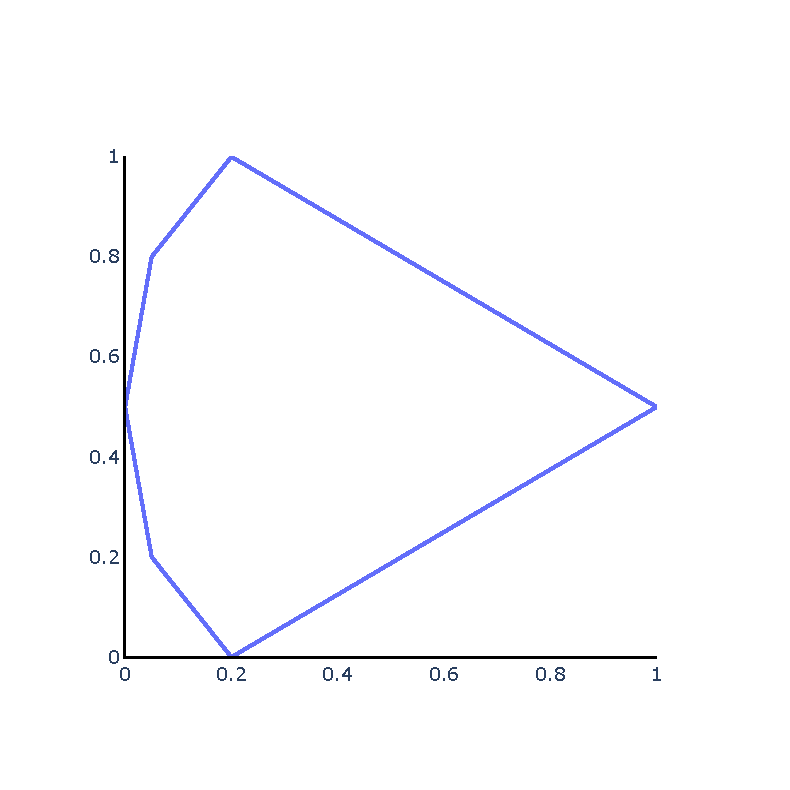
\includegraphics[width=1.\textwidth]{./Images/sampling_1}
		\caption{}
		\label{fig:sampling_1}
	\end{subfigure}%
	%\vspace{10pt}
	\begin{subfigure}{.45\textwidth}
		\centering
		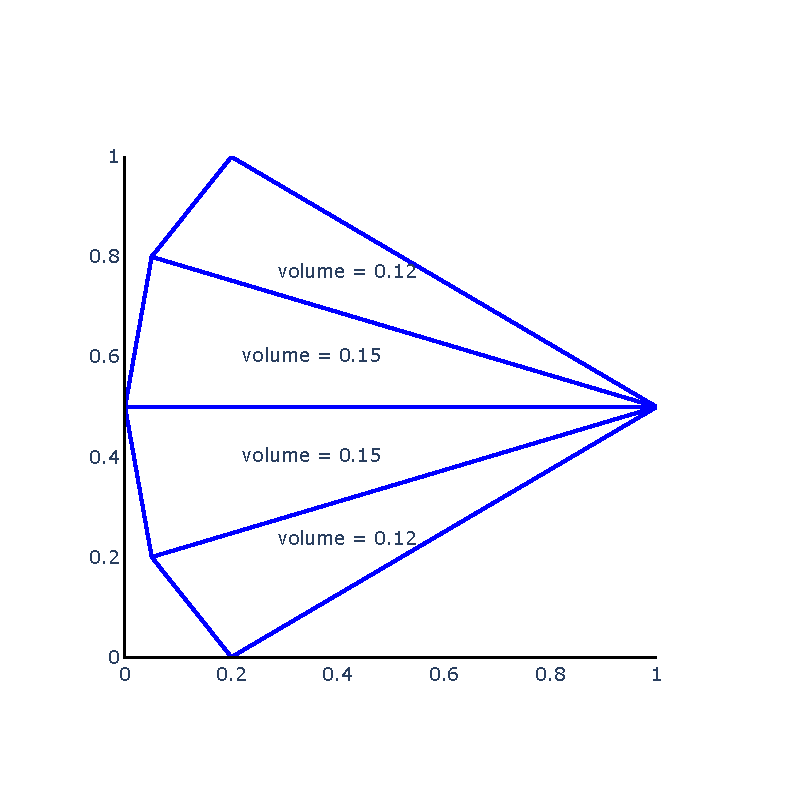
\includegraphics[width=1.\textwidth]{./Images/sampling_2}
		\caption{}
		\label{fig:sampling_2}
	\end{subfigure}
	\vspace{-10pt}
	\begin{subfigure}{.45\textwidth}
		\centering
		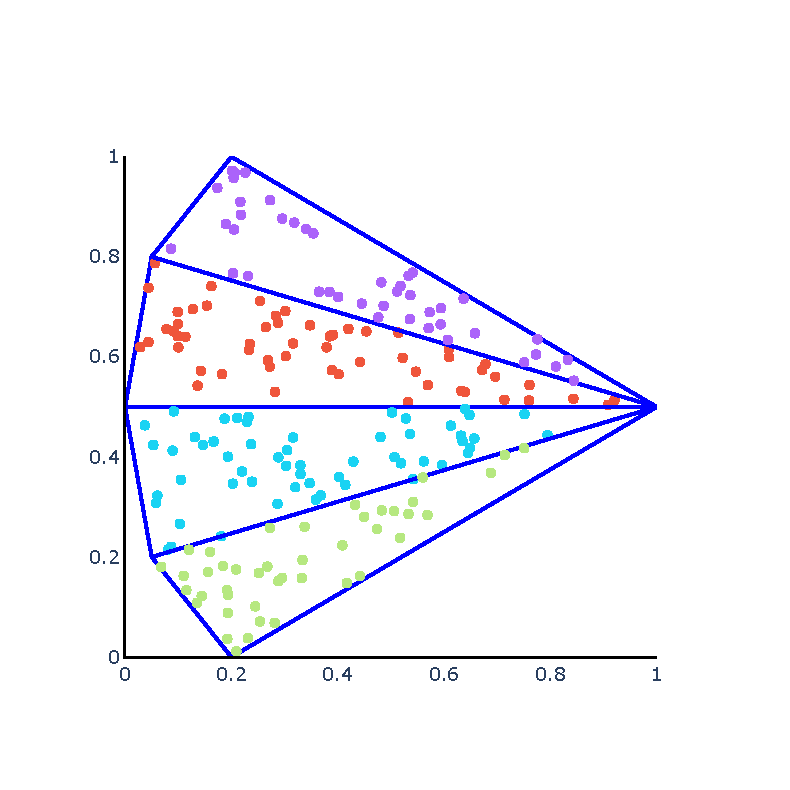
\includegraphics[width=1.\textwidth]{./Images/sampling_3}
		\caption{}
		\label{fig:sampling_3}
	\end{subfigure}%
	%\vspace{10pt}
	\begin{subfigure}{.45\textwidth}
		\centering
		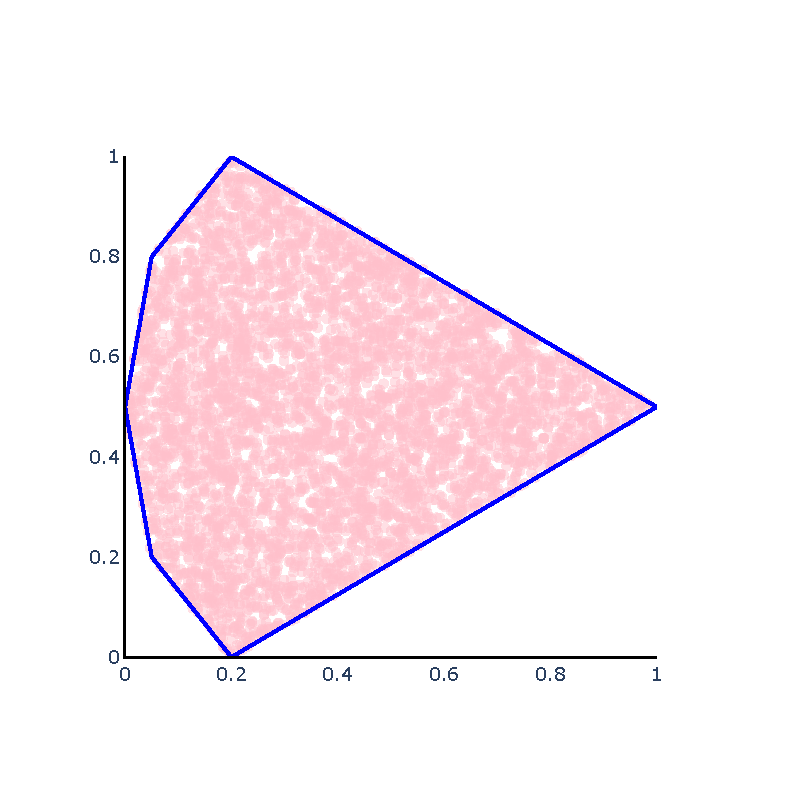
\includegraphics[width=1.\textwidth]{./Images/sampling_4}
		\caption{}
		\label{fig:sampling_4}
	\end{subfigure}
	\caption{An illustration of the sampling method. Figure (a)  shows the initial convex hull, figure (b) presents the hull separated into simplexes and their individual area. Figure (c) shows how 200 sample points are distributed between the individual simplexes, and figure (d) shows the final sampling with 5000 sample points evenly distributed over the convex hull.}
\end{figure}


Having sampled evenly across the entire convex hull approximating the near-optimal feasible space, a dataset containing all sample points is now available. These points can now be used to provide information about the distribution of variables and their correlations within this near-optimal feasible space. From the dataset, it is possible to find common features shared amongst all near-optimal solutions such as minimum capacity requirements of the individual technologies, etc. 


\section{Multiplicity }\label{sec:Multiplicity}

When grouping variables to reduce dimensionality as described in Section \ref{sec:dim_reduction}, a lot of information is lost. Especially one very feature of the distribution of solutions in the near-optimal feasible space is lost. In the fully dimensional decision space, where every variable/dimension correspondents to the capacity of one specific technology in a specific country, all solutions are evenly distributed. Essentially a point in this space describes a specific configuration of the European energy grid. 
When the variables are grouped by summation and a new decision space of lower dimension is formed, this property is lost, as a point in the reduced decision, space covers over a range of possible configurations of the energy grid. Instead of describing a specific configuration of the energy grid, a point in the reduced decision space describes a set of equality constraints that the energy grid must satisfy. 

If the decision space of the original problem $W$ has $d$ dimensions, corresponding to the $d$ variables in $\mathbf{x}$. When no equality constraints are introduced, the solution space $X$ is also of $d$ dimensions. For every equality constraint introduced the dimensionality of the solution space is reduced by one dimension. If $o$ equality constraints are introduced the dimension of the solution space becomes $d-o$, meaning that the solution space is a $d-o$ dimensional subspace of the decision space. 

In the solution space of the original problem, every element/point is unique and corresponds to a unique configuration of the European energy grid. When a new decision space is formed $Y$, by creating new variables $\mathbf{y(x)}$ consisting of sums of decision variables, this feature is lost. Instead of representing a single configuration of the European energy grid, a point  $\mathbf{y}$ in the reduced decision space, represents a range of configurations. 
A point $\mathbf{y}$ in $Y$, covers over a subset of the solution space in $X$ of dimension $n-o-k$, where $k$ is the dimension of $Y$. 

An example would be a three dimensional problem with the near-optimal feasible space $X$, variables $\mathbf{x}$ and constraints $\mathbf{f}_i(\mathbf{x})$. There are only inequality constraints, thus the dimension of the solution space $X$ is 3. 

\begin{equation}    
\mathbf{x} = 
\begin{bmatrix}
x_{1} \\
x_{2} \\
x_{3}
\end{bmatrix}
\end{equation}

\begin{equation}    
X = \{ \mathbf{x} | \mathbf{f}_i(\mathbf{x}) \leq 0  \}
\end{equation}

Where, a reduced decision space of two dimensions $Y$ with the variables  $\mathbf{y}$ is introduced to simplify the problem.

\begin{equation}\label{eq:y_variables}    
\mathbf{y} = 
\begin{bmatrix}
y_1 = x_1 + x_2 \\
y_2= x_3 
\end{bmatrix}
\end{equation}

\begin{equation}    
Y = \{ \mathbf{y}(\mathbf{x}) | \mathbf{f}_i(\mathbf{x}) \leq 0  \}
\end{equation}

In this case, where the full dimension solution space $X$ is three dimensional and the reduced decision space $Y$ is of two dimensions, a solution $y$ in the reduced decision space, corresponds to a one-dimensional subspace of the original solution space. In other words a solution in $Y$ represent all points in $X$ that satisfies the original constraints $f(x)\leq0$ and the two equality constraints $ x_1 + x_2 = y_1$ and $x_3 = y_2 $. 
There might only be a single point in $X$ that satisfies these constraints, or there might be infinitely many, but as all solutions in $Y$ must satisfy the same constraints as the solutions in $X$, there will be at least one solution. 


In broader terms, a point in a reduced decision space $Y$ of dimension $k$ represents a set of equality constraints, increasing the total number of equality constraints in the original problem. Therefore a point $\mathbf{y}$ in $Y$ represents a subspace of the solution space $X$ of dimension $n-o-k$. 

%A solution/point $\mathbf{y}$ in $Y$ would then correspond to all solutions in $X$ that satisfies the constraints $ x_1 + x_2 = y_1$ and $x_3 = y_2 $. Essentially a new equality constraint is introduced in $X$ for every dimension of $Y$. 
%There might only be one specific configuration of the network that satisfies these constraints, or there might be infinitely many, but as all solutions in $Y$ must satisfy the same constraints as the solutions in $X$, there will be at least one solution. 


%The facet representing the intersection of these hyperplanes will be of $n-m$ dimensions. A different way of think about it is as a series of $m$ equations with $n$ unknowns. The solution to such a problem would have $n-m$ unknowns. 


%In the case of a two dimensional subspace $Y$ and a three dimensional decision space $X$, the intersection will be $3-2=1$ dimensional. As a 1-facet in 3D space is a line, then a point in the subspace $Y$ must represent all solutions in $X$ that are located on the line given by $ x_1 + x_2 = y_1$ and $x_3 = y_2 $. 

Thus by using the novel MGA approach presented in Section \ref{sec:Novel_MGA} on the reduced problem to determine the shape of $Y$, and then sampling $Y$ evenly, would generate misleading results, as some of the sampled points represents a single or a few configurations of the energy network, and some sample points represent a vast amount of configurations of the energy network. In order to achieve correct results, the points sampled in $Y$, should be assigned a weight representing the size of the subspace of $X$ that the given solution in $Y$ spans. In the case of a three-dimensional solution space and a two-dimensional reduced decision space, the weight assigned to each sample point should be the length of the line in $X$ given by the constraints that specific point in $Y$ represents. 

A method for determining the size of the subspace of $X$ that a point in $Y$ spans must be established. 

The subspace of $X$ given by a point in $Y$ can be described through a parametric representation. Following the example from above, where the two equality constraints  $ x_1 + x_2 = y_1$ and $x_3 = y_2 $ is to be satisfied, the parametric representation of the 1-facet in the three-dimensional space $X$ can be found by selecting two points that satisfy the constraints. These two points could be selected as: 

\begin{equation*}
\mathbf{x}^1 = 
\begin{Bmatrix}
y_1 \\
0 \\
y_2
\end{Bmatrix}
\; , \; \mathbf{x}^2 = 
\begin{Bmatrix}
0 \\
y_1 \\
y_2
\end{Bmatrix}
\end{equation*}

Using these two points the parametric representation of the 1-facet can be written as:

\begin{equation}\label{eq:1-facet}
\mathbf{x} = \mathbf{x}^1 + t \left(\mathbf{x}^1-\mathbf{x}^2  \right)
=
\begin{Bmatrix}
y_1 \\
0 \\
y_2
\end{Bmatrix}
+t    
\begin{Bmatrix}
y_1 \\
-y_1 \\
0
\end{Bmatrix}    
\end{equation}

The size of the 1-facet could now be found by integrating over $t$. But as the boundaries of $t$ are unknown this is not an option. Instead, we can use MGA to find the span of the 1-facet combined with the knowledge of the direction of the 1-facet given by the vector $\mathbf{x}^1 - \mathbf{x}^2$. 

Performing a MGA study where the two equality constraints $ x_1 + x_2 = y_1$ and $x_3 = y_2 $, are included and the search directions is chosen as the positive direction of the 1-facet $\mathbf{n} = \mathbf{x}^1 - \mathbf{x}^2$ and the negative direction $\mathbf{n} = -(\mathbf{x}^1 - \mathbf{x}^2)$. This provides two points that defines the ends of the 1-facet, allowing the length to be calculated as the difference between these two points projected on to the direction vector $\mathbf{x}^1 - \mathbf{x}^2$.

This method can be expanded to any dimension of solution space and subspace. The parametric representation of the subspace of $X$ then becomes:

\begin{equation}
\mathbf{x} = \mathbf{x}_1 + \sum_{i=1}^{(n-k)} t_i (\mathbf{x}_1-\mathbf{x}_{i+1})
\end{equation}

The points $\mathbf{x}_i$ should be selected such that no more than two points are co-linear. Using the vectors  $(\mathbf{x}_1-\mathbf{x}_{i+1}) \; for \; i=1..(n-k)$ as search directions in an MGA study, and computing the size of the found facet, it is possible to determine the multiplicity factor. 

This method of determining multiplicity was implemented on a small scale experiment, showing the profound effects of neglecting multiplicity. It was however not implemented on the full-scale experiments performed in this project, due to its computational cost and complexity.  


\subsection{Multiplicity experiment}

To understand the effect of multiplicity, an experiment has been performed using a three-dimensional problem with near-optimal feasible space $X$ and the two-dimensional reduced decision space $Y$. The techno-economic model used is a simplified version of the full-scale model used in this project, including only two nodes (Denmark and Sweden) connected by a single transmission line. Sweden has two technologies available, wind turbines and gas turbines (OCGT). Denmark is only allowed to install wind power. A $\text{CO}_2$ constraint is enforced requiring a 60\% reduction in emissions compared to an unrestricted scenario.  The decision variables in $\mathbf{x}$ are:

\begin{equation}
\mathbf{x} = 
\begin{Bmatrix}
x_1: \text{DK wind} \\
x_2: \text{SE wind} \\
x_3: \text{SE OCGT}
\end{Bmatrix}
\end{equation}

The variables of $\mathbf{y}$, when grouped by technology type then becomes: 

\begin{equation}
\mathbf{y} = 
\begin{Bmatrix}
y_1: \text{DK wind} + \text{SE wind} \\
y_2: \text{SE OCGT}
\end{Bmatrix}
\end{equation}

Finding the shape of $Y$ using the MGA approach presented in Section  \ref{sec:Novel_MGA} and sampling the space uniformly, yields the results presented in Figure \ref{fig:multi_no_weights}. The shape of the reduced decision space $Y$ presented on Figure \ref{fig:multi_1}, is quite simple and indeed linear. The distributions of the sample points on Figure \ref{fig:multi_1} mimics the shape of $Y$, by being almost triangular. 


\begin{figure}[h]\centering
	\begin{subfigure}{.48\textwidth} \centering
		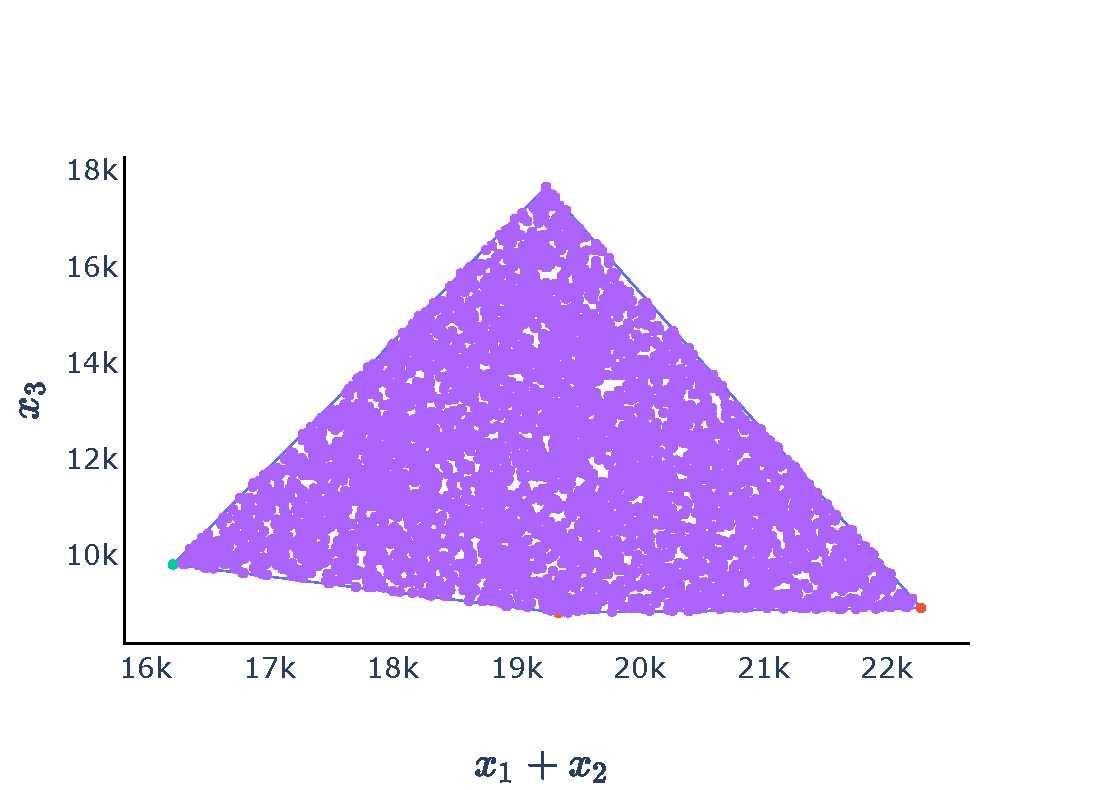
\includegraphics[width=1.\textwidth]{./Images/multi_1}
		\caption{}
		\label{fig:multi_1}
	\end{subfigure}
	\begin{subfigure}{.48\textwidth}  \centering
		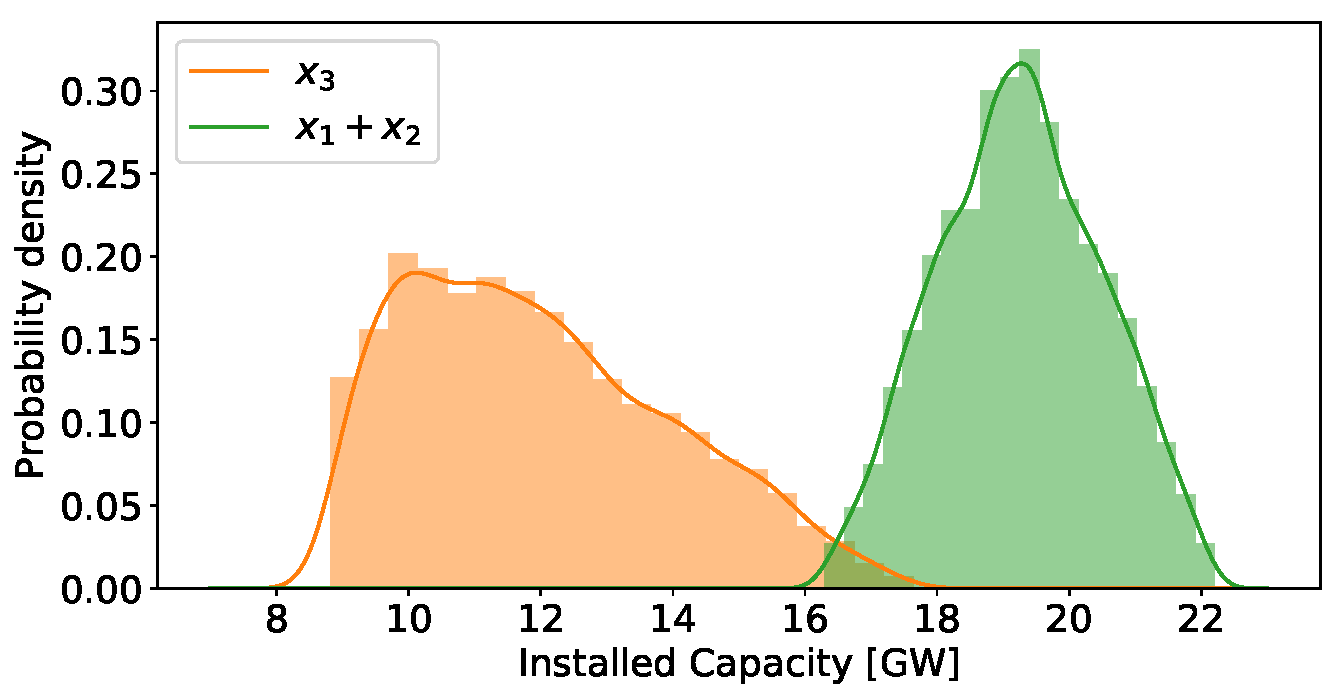
\includegraphics[width=1.\textwidth]{./Images/multi_2}
		\caption{}
		\label{fig:multi_2}
	\end{subfigure}
	\caption{The figure shows the results of a MGA study with grouped variables. Figure (a) shows the two dimensional subspace $Y$ and (b) presents a histogram of the sampled points from (a). }
	\label{fig:multi_no_weights}
\end{figure}


To generate a more realistic result, and to study the effect of multiplicity, the multiplicity for all sample points is evaluated. For every sample point, an MGA study of the full three-dimensional problem is performed with the two equality constraints from Equation \ref{eq:multi_constraint} introduced.

\begin{equation}\label{eq:multi_constraint}
\begin{split}
x_1 + x_2 &= y_1 \\
x_3 &= y_2
\end{split}
\end{equation}

The search directions for the objective function is chosen as $\mathbf{n}_1 = \{1,-1,0\}^T$ and  $\mathbf{n}_2 = -\{1,-1,0\}^T$. These two directions are chosen, by following the method proposed in Section \ref{sec:Multiplicity}, where a parametric representation of the subspace of $X$ given by a point in $Y$ is found, and the direction vector used as search direction. The weight of the individual points is then given by the area of the subspace of $X$ given by that specific point in $Y$. In this case, it is equivalent to the euclidean distance between the two points found by searching in the $\mathbf{n}_1$ and $\mathbf{n}_2$ direction. The weighted points are shown in Figure \ref{fig:multi_4}, and a histogram using the weighted points are shown in Figure \ref{fig:multi_5}. 

\begin{figure}[H]\centering
	\begin{subfigure}{.48\textwidth} \centering
		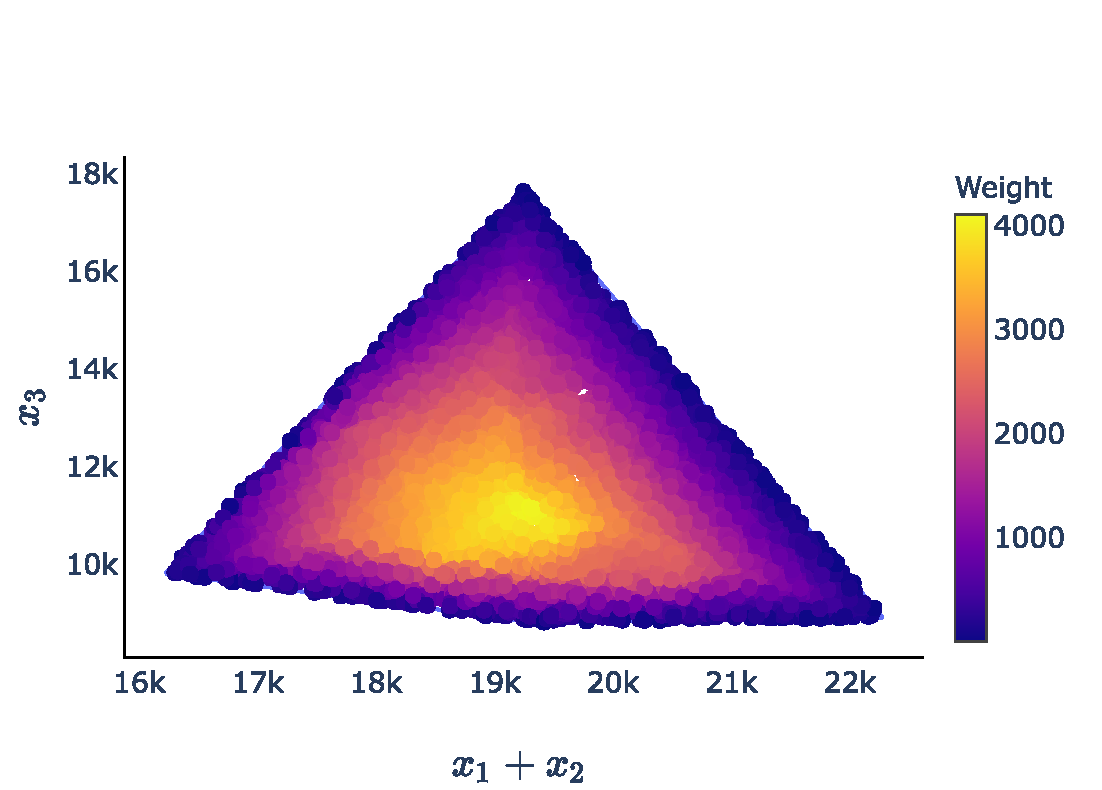
\includegraphics[width=1.\textwidth]{./Images/multi_4}
		\caption{}
		\label{fig:multi_4}
	\end{subfigure}
	\begin{subfigure}{.48\textwidth} \centering
		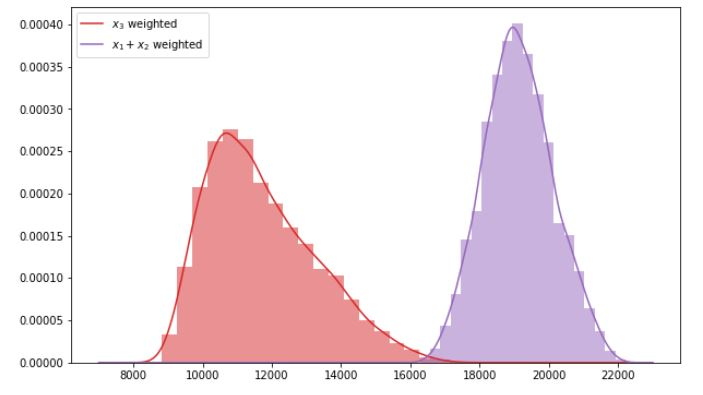
\includegraphics[width=1.\textwidth]{./Images/multi_5}
		\caption{}
		\label{fig:multi_5}
	\end{subfigure}
	\caption{MGA results of a study using grouped variables and a weighting of the sample points based on their multiplicity. Figure (a) shows the weighted sample points, and figure (b) shows a histogram of weighted sample points.}
\end{figure}

It is seen how the points closer to the center of the reduced decision space in Figure \ref{fig:multi_4}, is assigned a much higher weight than the points on the perimeter of the reduced decision space. This leads to the distributions being narrower and taller as seen in Figure \ref{fig:multi_5}. The distributions have now become more bell-curved, and the lower deviation suggests that scenarios located in the center of the reduced decision space are much more likely to occur than scenarios on the perimeter. 

To validate the results of the weighting method, an MGA study on the full problem is also performed. This study explorers the entire three-dimensional decision space and samples it evenly.
The results of this study is presented on Figure \ref{fig:multi_comparison}a and \ref{fig:multi_comparison}b, showing the three dimensional space $X$ on Figure \ref{fig:multi_6} and the distributions of the sampled points on Figure \ref{fig:multi_7}.  

\begin{figure}[h]\centering
	\begin{subfigure}{.5\textwidth} \centering
		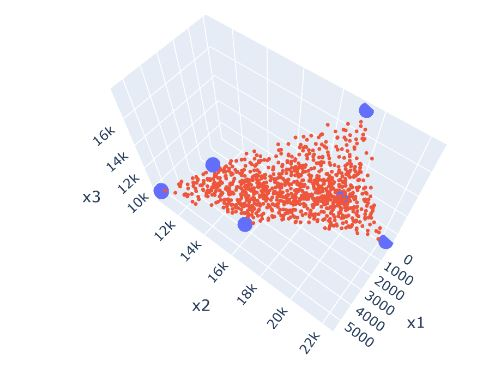
\includegraphics[width=1.\textwidth]{./Images/multi_6}
		\caption{}
		\label{fig:multi_6}
	\end{subfigure}%
	\begin{subfigure}{.5\textwidth} \centering
		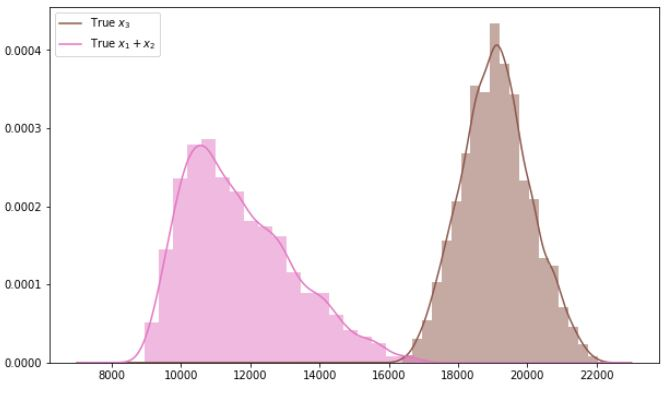
\includegraphics[width=1.\textwidth]{./Images/multi_7}
		\caption{}
		\label{fig:multi_7}
	\end{subfigure}%
	\vspace{10pt}
	\begin{subfigure}{.5\textwidth}
		\centering
		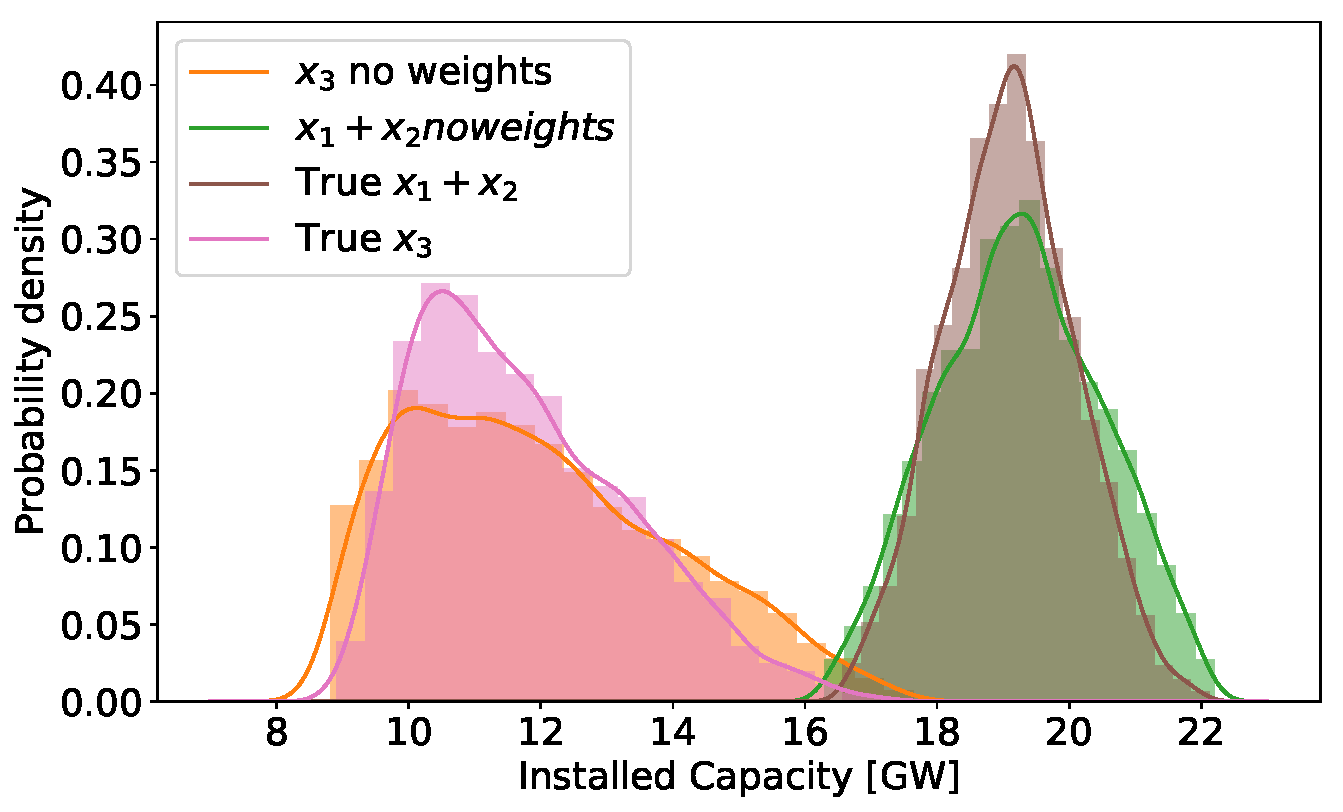
\includegraphics[width=1.\textwidth]{./Images/multi_8}
		\caption{}
		\label{fig:multi_8}
	\end{subfigure}%
	%\vspace{10pt}
	\begin{subfigure}{.5\textwidth}
		\centering
		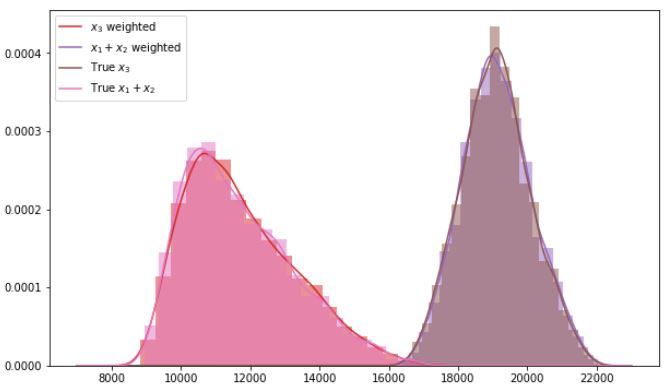
\includegraphics[width=1.\textwidth]{./Images/multi_9}
		\caption{}
		\label{fig:multi_9}
	\end{subfigure}
	\caption{Figure (a) and (b) show the result of an MGA study using three decision variables. In Figure (a) the three-dimensional near-optimal feasible space is presented and a histogram of the sampled point is seen on (b). Figure (c) and (d) compares the results found by performing MGA on the full three-dimensional decision space with the results of two MGA studies using grouped variables. In Figure (c), results from the three-dimensional study are compared to the MGA study of grouped variables, not weighting the sample points. On figure (d) the results from the three-dimensional study are compared to the MGA study of grouped variables weighting the sample points.}
	\label{fig:multi_comparison}
\end{figure}

The distributions of the sampled points from the approach without calculating the weights, and the one weighting the sample points are compared to the full solution on Figure \ref{fig:multi_comparison}. In Figure \ref{fig:multi_9} it is seen that the result using weighted points matches almost perfectly with the true solution. In practice, this means that, without the weighting, solutions too close to the frontier of the near-optimal solution space seem to be "similarly probable" as the solutions in the inner part of the near-optimal space when this is not true in reality. 
Consequently, when including the weighting, the probability density graphs squeeze, reducing the probability for extreme values. 


This insight is very important, as previously conducted MGA studies from literature \cite{DECAROLIS2016}, \cite{MGA_Price}, \cite{BERNTSEN2017886}, \cite{Yavuz2011}, \cite{Optimum_not_enough} and \cite{Fabian_MGA}, have had a tendency to focus on solutions located on the very perimeter of the decision space. When analyzing only the extreme points, it is important to remember that these solutions are unique, and no other configurations of the model can generate the same results. Wheres, when the entire decision space is sampled, it is possible to consider where the flexibility of the model lies. 

\subsection{Multiplicity in higher dimensions}

It is suspected that multiplicity become a larger factor as the dimensionality of the full problem increases. Therefore the multiplicity experiment have been repeated, with two new models with respectively 4 and 6 variables. The decision space of reduced dimension have been kept in two dimensions. The variables $\mathbf{x}$ in the two new experiments then becomes:

\begin{equation*}
\mathbf{x} = 
\begin{Bmatrix}
x_1:& \text{DK wind} \\
x_2:& \text{DK OCGT} \\
x_3:& \text{SE wind} \\
x_4:& \text{SE OCGT} 
\end{Bmatrix}
\; \text{and} \; 
\mathbf{x} = 
\begin{Bmatrix}
x_1:& \text{DK wind} \\
x_2:& \text{DK OCGT} \\
x_3:& \text{SE wind} \\
x_4:& \text{SE OCGT} \\
x_5:& \text{NO wind} \\
x_6:& \text{NO OCGT} 
\end{Bmatrix}
\end{equation*}

Grouping the variables by generator type, the variables of the reduced decision spaces become:

\begin{equation*}
\mathbf{y} = 
\begin{Bmatrix}
y_1: x_1 + x_3 \\
y_2: x_2 + x_4
\end{Bmatrix}
\; \text{and} \;
\mathbf{y} = 
\begin{Bmatrix}
y_1: x_1 + x_3 + x_5 \\
y_2: x_2 + x_4 + x_6
\end{Bmatrix}
\end{equation*}

Following the same method as used in the previous multiplicity study, where the MGA method is first used on the reduced decision space, without calculating the weights of the points, and then weighting all the sample points. Both results are compared to the true solution, found by performing an MGA study on the full-dimensional problem. 

\begin{figure}[hb]\centering
	\begin{subfigure}{.5\textwidth}
		\centering
		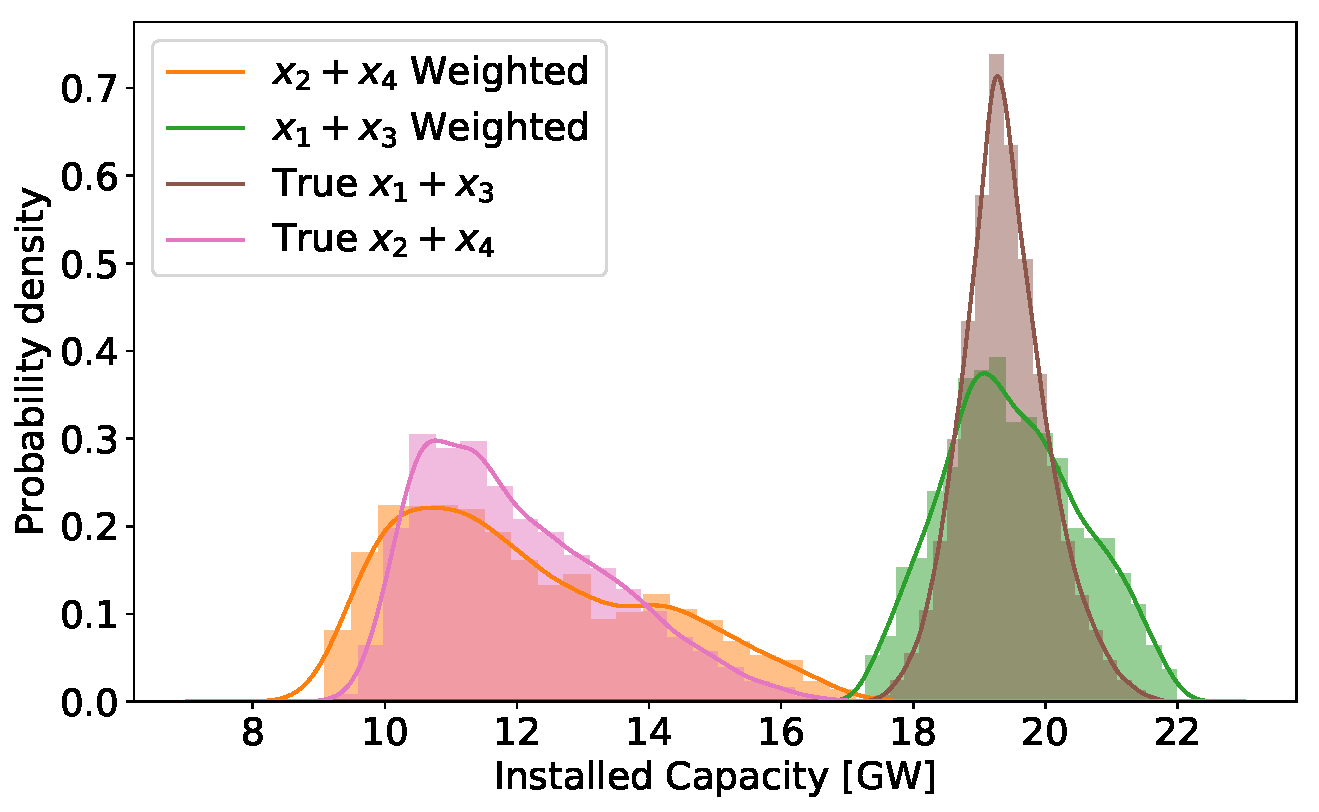
\includegraphics[width=1.\textwidth]{./Images/multi_4D_1}
		\caption{}
		\label{fig:multi_4D_1}
	\end{subfigure}%
	%\vspace{10pt}
	\begin{subfigure}{.5\textwidth}
		\centering
		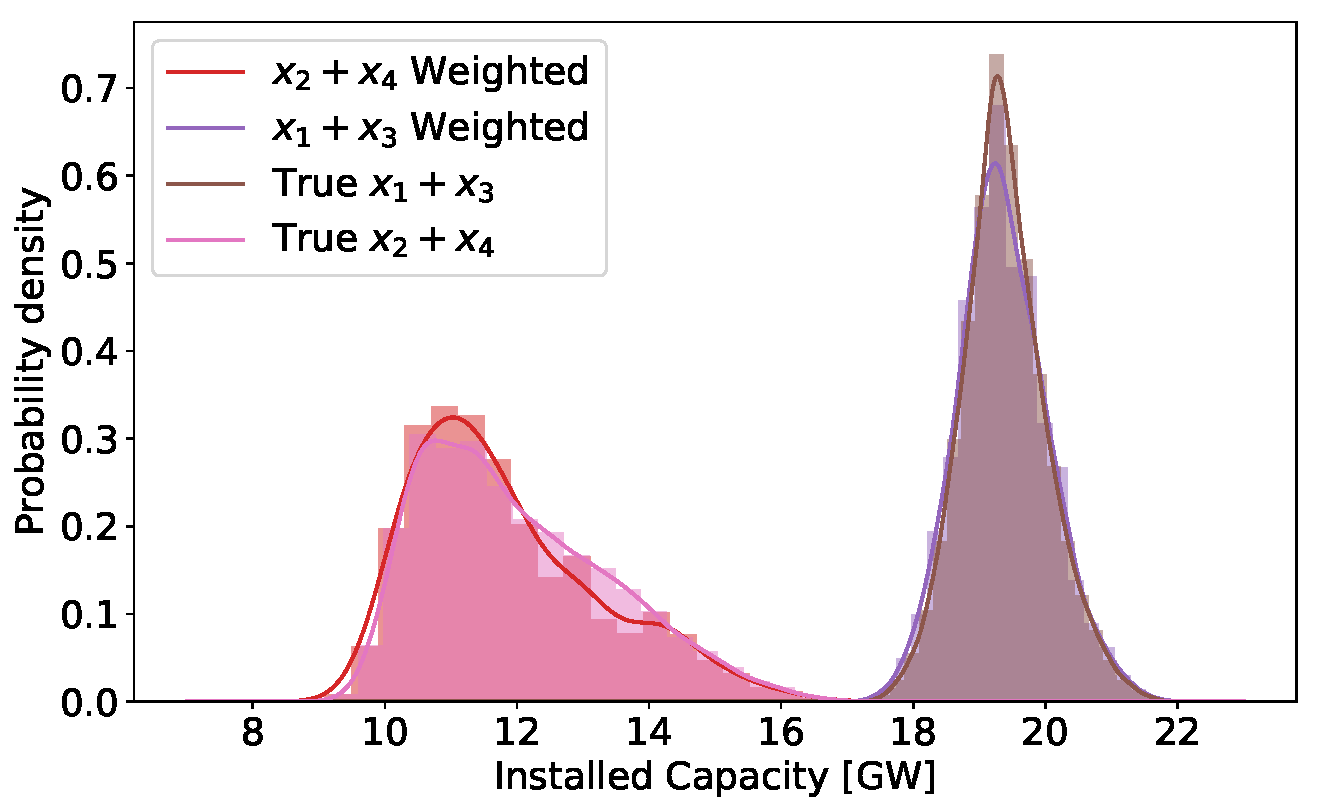
\includegraphics[width=1.\textwidth]{./Images/multi_4D_2}
		\caption{}
		\label{fig:multi_4D_2}
	\end{subfigure}
	\vspace{10pt}
	\begin{subfigure}{.5\textwidth}
		\centering
		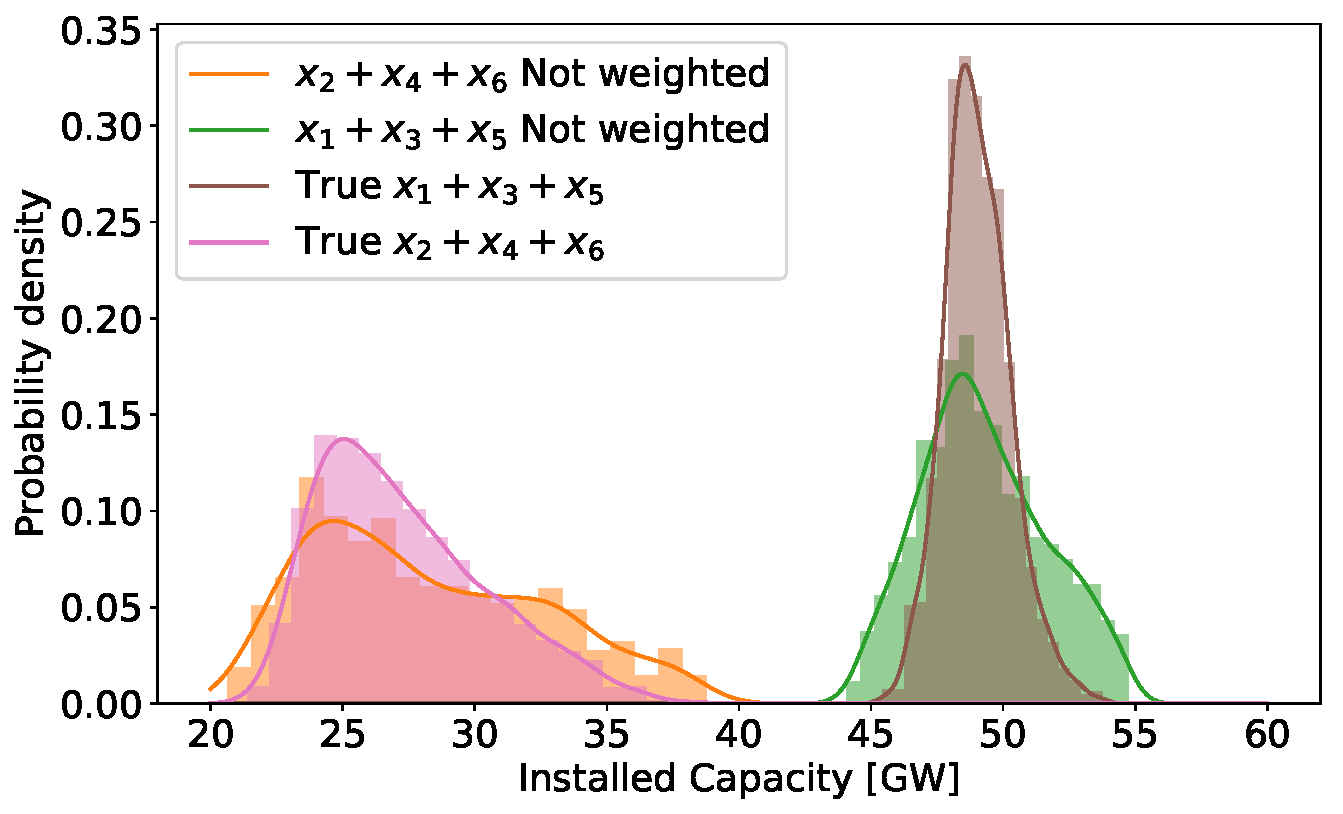
\includegraphics[width=1.\textwidth]{./Images/multi_6D_1}
		\caption{}
		\label{fig:multi_6D_1}
	\end{subfigure}%
	%\vspace{10pt}
	\begin{subfigure}{.5\textwidth}
		\centering
		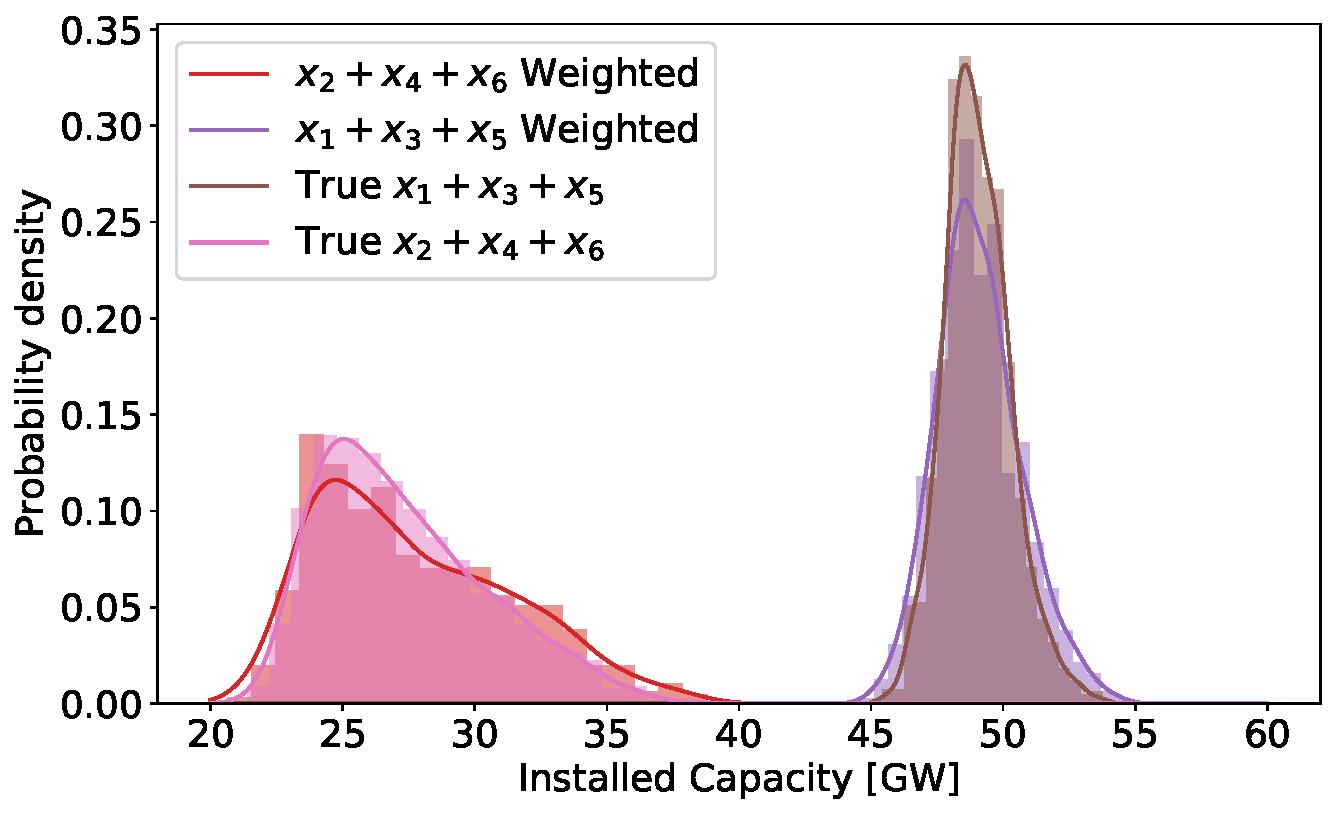
\includegraphics[width=1.\textwidth]{./Images/multi_6D_2}
		\caption{}
		\label{fig:multi_6D_2}
	\end{subfigure}
	\caption{Figure (a) and (b) presents the results from a four dimensional study with a reduced decision space of two dimensions. Figure (c) and (d) shows the results a six dimensional study with a reduced decision space of two dimensions}
	\label{fig:multi_46D}
\end{figure}

In Figure \ref{fig:multi_46D}, the results from the four and six-dimensional problems are presented. Comparing the not weighted, solution from the four-dimensional problem seen on Figure \ref{fig:multi_46D}a, to the not weighted solution for the three-dimensional study on Figure \ref{fig:multi_comparison}, it is seen that a larger mismatch between the true solution and the estimated one, occurs as the dimension increases. Extending this analysis to the six-dimensional problem seen in Figure \ref{fig:multi_46D}c, it is seen that this trend continues. 
However, comparing the weighted approaches in all three studies seen in Figure \ref{fig:multi_comparison}b and Figure \ref{fig:multi_46D}b and \ref{fig:multi_46D}d, a much better fit between the distributions is found. These results suggest that the proposed method of estimating multiplicity is working correctly. 


Estimating the effect of multiplicity in this manner is however not feasible for larger problems. Every estimation of a sample point weight essentially requires an MGA study on its own, and as more than 1000 sample points are needed to generate well-representing results, the computational effort needed becomes too high. Instead of using the approach for estimating multiplicity presented in this section, as a tool to use in larger simulations, this study should serve as a proof and reminder, that the true distribution of solutions is much narrower than what is found when using MGA algorithms, on a reduced dimensional decision space. 


\section{Gini coefficient}

The goal of this project is to develop a method to deal with structural uncertainty in techno-economic energy models, arising from unmodeled objectives. One very important factor that isn't included in the objective function is the equality in average yearly production versus consumption. In a model including multiple countries, like the one used in this project, this could be very important as countries in general desire to be somewhat self-sufficient with energy. 

To create a measure for the equality of production versus consumption, the Gini coefficient can be used. Calculating the cumulative share of demand per country and plotting it against the cumulative share of generation per country one gets the Lorentz curve for that specific scenario, as shown for four scenarios in Figure \ref{fig:Gini_2}. As inequality increases the Lorentz curve lies further and further away from the equality line. 

The Gini coefficient is calculated as the relationship between the area between the Lorentz curve and the equality line (Area A on Figure \ref{fig:Gini_1}) relative to the total area under the equality line  (Area A+B on Figure \ref{fig:Gini_1}). Thus the Gini coefficient becomes $G = \frac{A}{A+B}$.

\begin{figure}[h]\centering
	\begin{subfigure}{.5\textwidth}
		\centering
		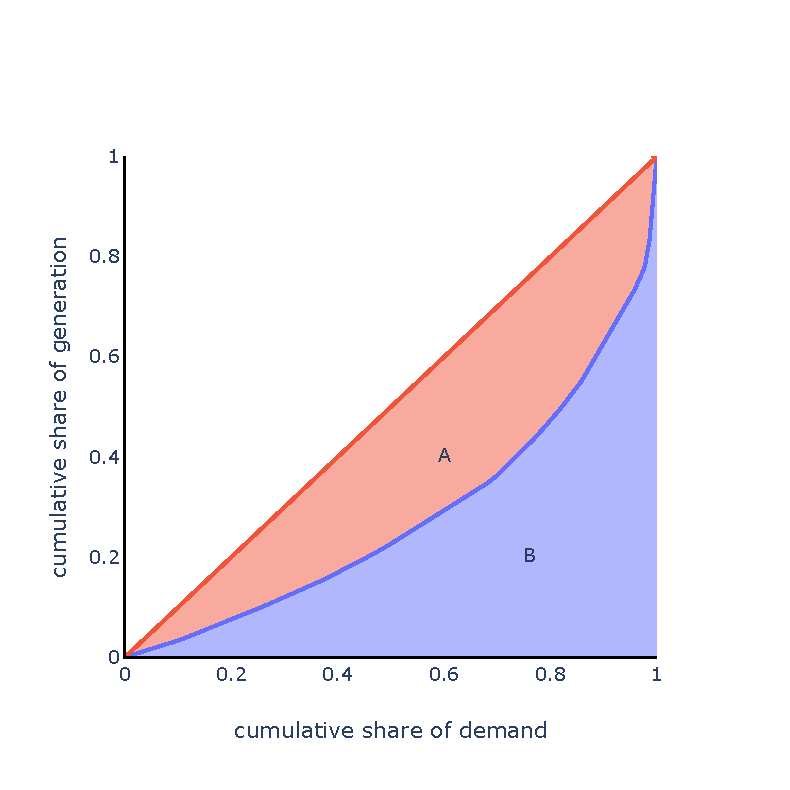
\includegraphics[width=1.\textwidth]{./Images/Gini_1}
		\caption{}
		\label{fig:Gini_1}
	\end{subfigure}%
	%\vspace{10pt}
	\begin{subfigure}{.5\textwidth}
		\centering
		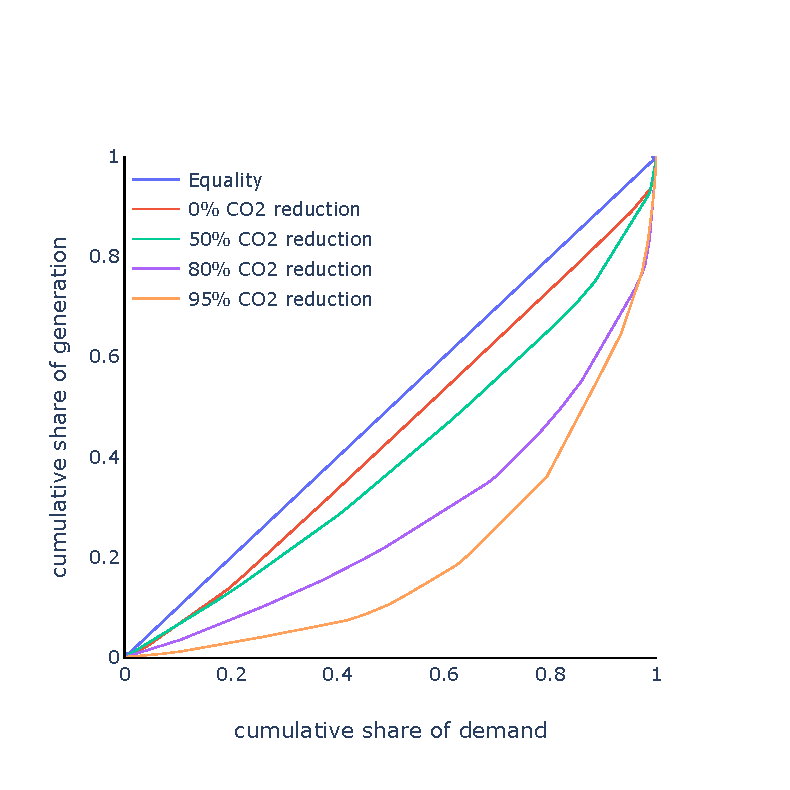
\includegraphics[width=1.\textwidth]{./Images/Gini_2}
		\caption{}
		\label{fig:Gini_2}
	\end{subfigure}
	\caption{On figure (a), a schematic of the areas considered when calculating the Gini coefficient is presented. Figure (b), shows the Lorentz curves of four studies using different CO2 constraints.}
	\label{fig:Gini}
\end{figure}

A scenario where every country over the duration of an entire year, produces as much energy as it consumes, would have a Gini coefficient of 0, and represent the equality line on Figure \ref{fig:Gini}. A scenario where one country is producing all energy and consuming none, would, on the other hand, have a Gini coefficient of 1, and represent total inequality. 

The Gini coefficient calculated in this manner is a very good measure of the distribution of energy production versus consumption. As a very important unmodeled objective in a techno-economic energy model including multiple countries, is the desire for the countries to be self-sufficient, this Gini coefficient provides a very important insight.



